% **************************************************
% Document class
% **************************************************

\documentclass[
	a4paper,
	12pt,
	bibtotoc,
	listof=totoc,
	titlepage
]{scrartcl}


% **************************************************
% Settings
% **************************************************

\usepackage{settings}


% **************************************************
% Variables
% **************************************************

\newcommand*{\getUniversity}{Hochschule für angewandte Wissenschaften München}
\newcommand*{\getFaculty}{Fakultät für Informatik und Mathematik}
\newcommand*{\getTitle}{Implementierung eines Drahtlosen Fußschalters}
\newcommand*{\getAuthor}{Wolfram Barth}
\newcommand*{\getMatriculationNumber}{03708119}
\newcommand*{\getCourse}{Informatik}
\newcommand*{\getDoctype}{Bachelorarbeit}
\newcommand*{\getSupervisor}{Prof. Dr. Stefan Wallentowitz}
\newcommand*{\getSubmissionDate}{\today}


% **************************************************
% PDF Metadata
% **************************************************

\hypersetup{
	pdftitle = \getTitle,
	pdfauthor = \getAuthor,
	pdfsubject = \getDoctype
	pdfkeywords = {Bachelorarbeit, Informatik}
}


% **************************************************
% Content
% **************************************************

\begin{document}

\titlehead{
	\begin{flushright}
		
\includegraphics[width=50mm]{logos/university_logo}
	\end{flushright}
	\begin{center}
		{\Large \getUniversity}\\
		{\large \getFaculty}
		\vspace*{10mm}
	\end{center}
}

\subject{\getDoctype\ zum Thema:}

\title{\vspace{-10mm} \getTitle}

\subtitle{Zur Erlangung des akademischen Grades Bachelor of Science}

\author{}

\date{}

\publishers{
	\parbox{\textwidth}{
		\vspace*{40mm}
		\large
		\begin{tabularx}{0.8\textwidth}{lX}
			\textbf{Vorgelegt von:} & \getAuthor \\[0.7em]
			\textbf{Matrikelnummer:} & \getMatriculationNumber \\[0.7em]
			\textbf{Studiengang:} & \getCourse \\[0.7em]
			\textbf{Betreuer:} & \getSupervisor \\[0.7em]
			\textbf{Abgabedatum:} & \getSubmissionDate \\[0.7em]
		\end{tabularx}
	}
}\normalsize

\maketitle

\begin{abstract}

\section*{Abstract}
Die Digitalisierung von Hand- und Messwerkzeugen in der Industrie führt dazu, dass eine steigende Menge an Daten zusammengeführt und verarbeitet werden muss. Sie werden dazu in speziellen Formaten benötigt, weshalb entweder Software- oder Hardware-Lösungen für die Umwandlung von Nöten sind. Während die Software-Lösungen, aufgrund der hohen Sicherheitsrichtlinien in der industriellen Fertigung, zeitaufwändige und komplexe Einführungsprozesse nachsichziehen, gibt es noch keine Hardware-Lösungen, welche sowohl die Umwandlung in die benötigten Formaten, als auch die kabellose Anbindung des Hand- und Messwerkzeugen übernimmt. Dabei wird die folgende Forschungsfrage gestellt: Wie sollten die Software- und Hardware-Komponenten eines intelligenten Fußschalters gestaltet werden, damit dieser ohne die Installation weiterer Software Hand- und Messwerkzeug an ein Computersystem kabellose anbindet und deren Messergebisse in verschiedenen konfigurierbaren Formaten zur Verfügung stellt? Es wird auf einem intelligenten Fußschalter, als auch auf einem USB-Dongle, eine Anwendung entwickelt, welche die Daten von Messwerkzeugen zusammenführt und für die Weiterverarbeitung aufbereitet. Diese Anwendung stellt einen neuen softwarebasierten Ansatz da, wie industrielle Hand- und Messwerkzeug an einen Computer angebunden werden kann und die Messdaten verarbeitet werden können. Sie kann von der Industrie dazu verwendet werden um darauf aufbauend konkrete Produkte zu entwickeln. So wird die Hoffmann Group, für deren Werkzeug exemplarisch die Implementierung durchgeführt wurde, den Fußschalter und USB-Dongle in ihr Produktportfolio aufnehmen. Die Ergebnisse der Entwicklung werden evaluiert und werden von der Forschung dazu verwendet, um weitere Konzepte zur Anbindung von Werkzeugen an Computer zu entwickeln.

\end{abstract}

\tableofcontents

\clearpage
\listoffigures

\clearpage
\listoftables

\clearpage
\lstlistoflistings

\clearpage
\section*{Abkürzungsverzeichnis\markboth{Abkürzungsverzeichnis}{}}
\addcontentsline{toc}{section}{Abkürzungsverzeichnis}

\begin{acronym}[CI]

\acro{HCT}[HCT]{Hoffmann connected tools}
\acro{BLE}[BLE]{Bluetooth low energy}
\acro{HID}[HID]{Human interface device}
\acro{MSC}[MSC]{Mass storage class}
\acro{CSV}[CSV]{Comma seperated values}
\acro{CAQ}[CAQ]{Computer-aided quality assurance}
\acro{FIFO}[FIFO]{First in first out}
\acro{FAT}[FAT]{File allocation Table}
\acro{USB}[USB]{Universal Serial Bus}
\acro{UART}[UART]{Universal Asynchronous Receiver Transmitter}
\acro{LED}[LED]{light-emitting diode}
\acro{IDE}[IDE]{Integrated Development Environment}

\end{acronym}

\clearpage
\section{Einleitung}
In diesem Kapitel wird zunächst vorgestellt, mit welchen Geräten der Fußschalter interagiert und die zusammen die \ac{HCT}-Plattform bilden. Es wird gezeigt, wie sich der Fußschalter in diese Plattform einfügt, sowie Motivation der Implementierung erklärt.

\subsection{HCT-Plattform}
Die Digitalisierung von Werkzeug in der Industrie ist in vollem Gange. Der Hauptgrund dafür ist, neben der einfacheren und genaueren Bedienung, die Möglichkeit durchgeführte Arbeitsschritte auf einem Computer automatisiert zu protokollieren. Wurden früher Messergebnisse per Hand vom Werkzeug auf Papier übertragen, werden sie nun zuverlässig und fehlerfrei mit Bluetooth an einen Computer übertragen. Das steigert die Effizienz und ermöglicht die Automatisierung der Qualitätskontrolle, sowie den Nachweis, dass Standards in der Fertigung eingehalten wurden, was in Branchen wie der Automobilindustrie oder der Luftfahrt von großer Bedeutung ist. \\
Dabei wurde sich für \ac{BLE} enschieden, da den Hand- und Messwerkzeugen, aufgrund ihrer handlichkeit und nicht kabelgebundenheit, nur begrenzte Batteriespeicherkapazitäten zu Verfügung stehen. \ac{BLE} ist eine Abwandlung des klassischen Bluetooth und ist besonders auf Energiesparkeit hin optimiert, wodurch es auch auf dem Hand- und Messwerkzeug lange Batterielaufzeiten garantieren kann.\\
Um die Digitalisierung der Messergebnisse dem Anwender so einfach wie möglich zu gestalten, setzt die Hoffmann Group mit der HCT-Plattform darauf, die Digitalisierung der durchgeführten Arbeitsschritte als einen festen Bestandteil in ihr Werkzeug zu integrieren. Diese sind zum Stand dieser Arbeit: 
\begin{itemize}
	\item Drehmomentschlüssel
	\item Messschieber bzw. Messuhren
	\item Drehmomentprüfgerät
\end{itemize}
Sie stellen dem Anwender die Daten der Messungen in verschiedener Weise zu Verfügung. Zum Einen können die Geräte als ein \ac{HID} über \ac{BLE} mit dem Computer verbunden werden. Sie simulieren dann eine über Bluetooth verbundene Tastatur über die, die Messergebnisse als Tastendrücke serialisiert werden. Das Messergebnis kann dann in einem Texteditor oder Excel aufgefangen werden. Des weiteren erzeugen die Drehmomentschlüssel und das Drehmomentprüfgerät eine \ac{CSV}-Datei, in der alle durchgeführten Messungen mit einer großen Anzahl an zusätzlichen Daten gespeichert werden. Wird das Gerät über \ac{USB} mit dem Computer verbunden, zeigt es sich als \ac{MSC}-Device und die Datei kann per Drag-and-drop auf den Computer kopiert werden. Die letzte Möglichkeit die durchgeführten Messungen zu digitalisieren, ist mithilfe der \ac{HCT}-Windows-App. Diese erfordert zusätzlich zur frei verfügbaren Software einen speziellen Dongle der zum Verbinden der Geräte benötigt wird. Sie werden ebenfalls über \ac{BLE} verbunden und sprechen über \ac{BLE} das firmeneigene \ac{HCT}-Protokoll. Die Windows-App bietet zahlreiche Möglichkeiten die Messdaten zu digitalisieren und den Produktionsprozess zu optimieren. Es können Schraubfälle in der App angelegt werden und mit Bildern hinterlegt werden. Die Seriennummer von Werkstücken kann automatisch mit dem dazugehörigen Messwert verlinkt werden und \ac{CAQ}-Software kann über einen virtuelle COM-Port angebunden werden. Die \ac{HCT}-Windows-App unterstützt derzeit lediglich die Drehmomentschlüssel, jedoch ist die Einbindung der restlichen \ac{HCT}-Geräte in Entwicklung. Der letzte Baustein der \ac{HCT}-Plattform ist die \ac{HCT}-Mobile-App, sie ist ebenfalls frei erhältlich und erleichtert vorallem die Bedienung des Geräts, zum Beispiel bei Arbeitsschritten bei denen das Display des Werkzeugs für den Anwender nicht sichtbar ist.

\subsection{HCT-Protokoll}
Der \ac{HCT}-Plattform liegt das firmeneigene \ac{HCT}-Protokoll zugrunde. Es stellt sicher, dass alle Geräte der \ac{HCT}-Plattform stets kompatibel zu einander sind. Es ist ein binäres Protokoll, dass entwickelt wurde um über \ac{BLE} gesprochen zu werden und stellt ein virtuelles Speichermodel der Geräte da. Dabei besitzten Werkzeuge unterschiedlicher Produktreihen und Hersteller jeweils verschiedene Speichermodelle. Über ``read'' und ``write'' Befehle auf die Speicheradressen kann dann der interne Zustand des Werkzeug abgefragt und verändert werden. So können auch komplexe Operationen effizient über \ac{BLE} durchgeführt werden. Zudem stehen automatisierte Tools zur Verfügung mit deren Hilfe die Frameworks, die das Sprechen des HCT-Protokoll abstrahieren, um die Speichermodelle neu eingeführter Werkzeuge erweitert werden kann.
\begin{figure}[H] 
	\centering
	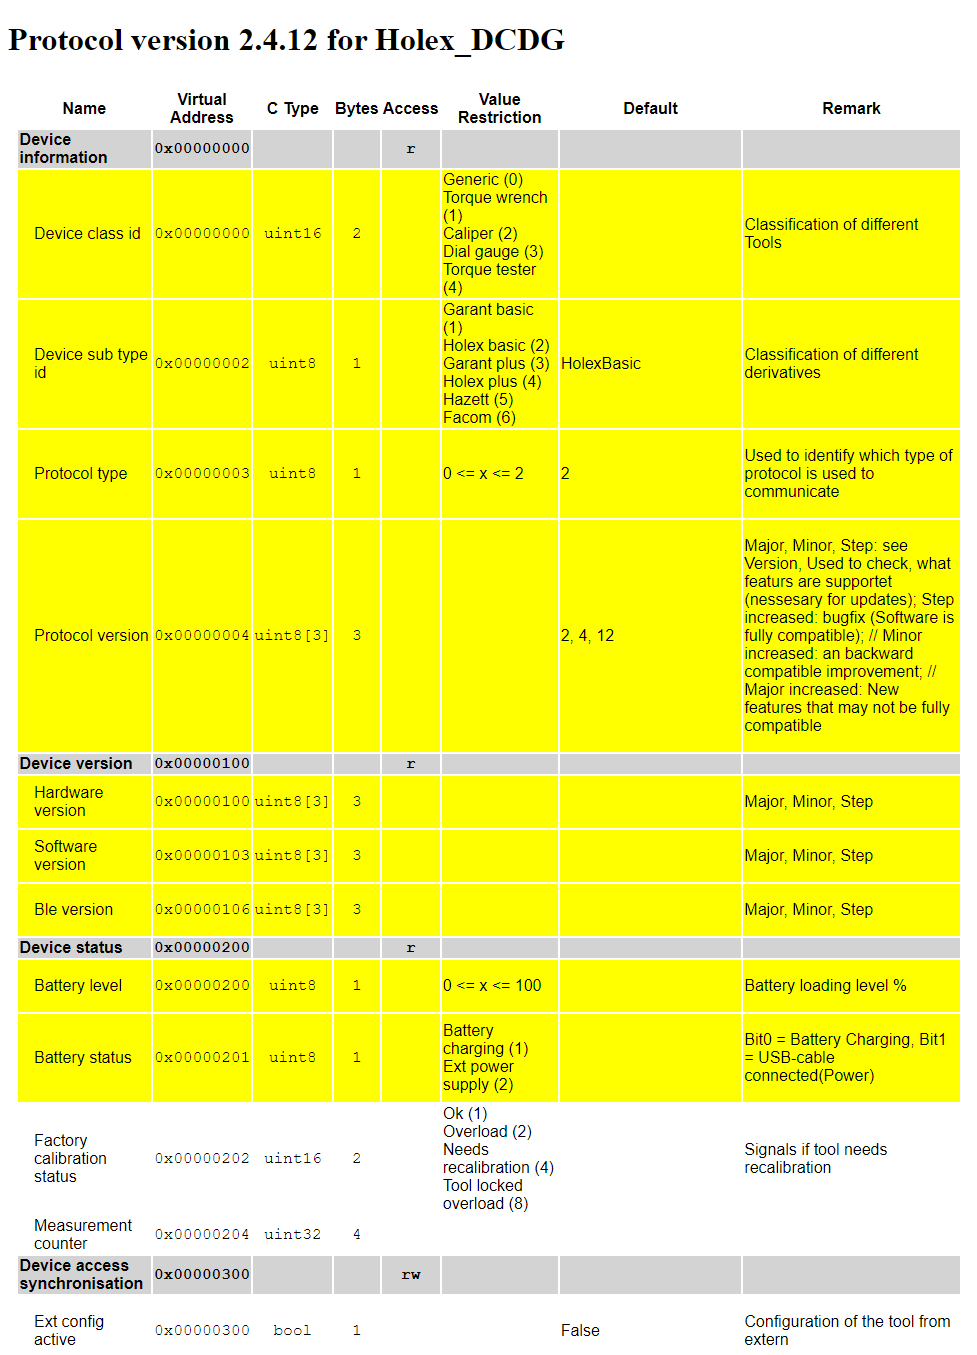
\includegraphics[width=\textwidth]{figures/HCT_Protocol_DCDG.png}
	\caption{Auszug aus \ac{HCT}-Protokoll für Messuhren und Messschieber}
\end{figure}

\subsection{Motivation}
Es hat sich gezeigt, dass die Einführung der \ac{HCT}-Windows-App immer wieder auf großen Widerstand von IT-Abteilungen trifft. Diese haben Sicherheitsbedenken, da die App direkt in der Fertigung eingesetzt wird und es müssen daher langwierige interne Prozesse für die Einführung angestoßen werden. Der Fußschalter soll ohne einer Installation die Funktion der Windows-App, die Serialisierung von Messergebnisse über einen virtuelle COM-Port im MUX50 bzw. DMX16-Protokoll, zur Verfügung stellen. \\
Des weiteren muss zum Senden eines Messwerts an den Computer bei Messschiebern und Messuhren eine Taste gedrückt werden. Bei der Durchführung von hochpräzisen Messungen, die auf den hundertstel Millimeter genau sein müssen, verfälscht dieses Betätigen einer Taste auf dem Gerät jedoch bereits die Messung. Auch bei der Durchführung von möglichst zeitgleichen Messungen mit mehreren Messgeräten stellt das Drücken einer Taste zum Senden des Messwerts den Nutzer vor Pro\ac{BLE}me. Daher werden in der Industrie Fußschalter eingesetzt, die kabelgebunden sowohl an das Werkzeug als auch an den Computer, dieses Senden der Messung auslösen können. Durch die kabelgebundene Natur dieser Fußschalter ist jedoch deren Einsatzbereich reduziert, da es nicht gegeben ist, dass in den Fertigungshallen und Werkstätten, in denen die Fußschalter eingesetzt werden, sich ein Computer in nächster Nähe befindet. Durch die Entwicklung eines Fußschalters der sich über Bluetooth mit dem Messwerkzeug verbindet, wird der Einsatzbereich deutlich vergrößert und der Einsatz dem Anwender erleichtert.

\clearpage
\section{Ausgangszustand}
Zum Beginn dieser Arbeit wurde bereits in meiner vorangegangen Tätigkeit bei Hoffmann Group auf Basis des NRF52840-Dongle prototypisch eine Anwendung implementiert, die auf das Bluetooth Modul der Hoffmann Group aufbaut und in der Lage ist sich selbstständig mit mehreren Drehmomentschlüsseln zu verbinden. Sie stellt die Messergebnisse bereits über einen virtuellen COM-Port im MUX50 bzw. DMX16 Protokoll zur Verfügung und die zu verbindenden Geräte sind über eine CSV-Datei, die über MSC dem Nutzer zur Verfügung gestellt wird, konfigurierbar.

\subsection{Aufbau}


\clearpage
\printbibliography

\clearpage
\begin{abstract}

\section*{Selbstständigkeitserklärung}
Hiermit erkläre ich, dass ich die Bachelorarbeit selbständig verfasst, noch nicht anderweitig für Prüfungszwecke vorgelegt, keine anderen als die angegebenen Quellen oder Hilfsmittel benutzt sowie wörtliche und sinngemäße Zitate als solche gekennzeichnet habe.\\

\bigbreak
\bigbreak

München, den \today

\end{abstract}

\end{document}